\documentclass[11pt]{article}
\usepackage[utf8]{inputenc}
\usepackage{verbatim}
\usepackage{subfig}
\usepackage{makeidx}
\usepackage{listings}
\usepackage{color}
\usepackage{tikz}
\usetikzlibrary{arrows}
\usepackage{pgf}
\usepackage{fancybox}
\usepackage{verbatim}
\usepackage{wrapfig}
\usepackage{graphicx}
\usepackage{hyperref}

\newcommand{\bigstar}{\mathop{\Huge \mathlarger{\mathlarger{*}}}}


\definecolor{dkgreen}{rgb}{0,0.6,0}
\definecolor{gray}{rgb}{0.5,0.5,0.5}
\definecolor{mauve}{rgb}{0.58,0,0.82}

\lstset{ %
  language=Octave,                % the language of the code
  basicstyle=\footnotesize,           % the size of the fonts that are used for the code
  numbers=left,                   % where to put the line-numbers
  numberstyle=\tiny\color{gray},  % the style that is used for the line-numbers
  stepnumber=2,                   % the step between two line-numbers. If it's 1, each line
  % will be numbered
  numbersep=5pt,                  % how far the line-numbers are from the code
  backgroundcolor=\color{white},      % choose the background color. You must add \usepackage{color}
  showspaces=false,               % show spaces adding particular underscores
  showstringspaces=false,         % underline spaces within strings
  showtabs=false,                 % show tabs within strings adding particular underscores
  frame=single,                   % adds a frame around the code
  rulecolor=\color{black},        % if not set, the frame-color may be changed on line-breaks within not-black text (e.g. commens (green here))
  tabsize=2,                      % sets default tabsize to 2 spaces
  captionpos=b,                   % sets the caption-position to bottom
  breaklines=true,                % sets automatic line breaking
  breakatwhitespace=false,        % sets if automatic breaks should only happen at whitespace
  title=\lstname,                   % show the filename of files included with \lstinputlisting;
  % also try caption instead of title
  keywordstyle=\color{blue},          % keyword style
  commentstyle=\color{dkgreen},       % comment style
  stringstyle=\color{mauve},         % string literal style
  escapeinside={\%*}{*)},            % if you want to add LaTeX within your code
  morekeywords={*,...}               % if you want to add more keywords to the set
}

% If you add the above paragraph, the following can be used to alter the settings within the code:
% \lstset{language=C,caption={Descriptive Caption Text},label=DescriptiveLabel}


\title{Specialization Project \\ A closer look at deep artificial neural networks}
\author{Lars Andersen \\
Tormund S. Haus}
\date{\today}
\begin{document}
\maketitle
\newpage
\tableofcontents

\clearpage
\section{Introduction}

This report details the work done this semester in the specialization project.  The goal of the project was to investigate deep belief networks. Specifically, to implement a deep belief network (DBN), using restricted Boltzman machines (RBM) as building blocks.  Implementing these networks, based on scientific papers, proved to be a much larger challenge than expected.  Instead of writing exclusively about a failed implementation attempt, we're also writing up a review of some of the interesting technologies we encountered during the semester.  At the beginning of the semester we had decided that these networks were interesting enough, in our eyes, that we wanted to work with them for a full year.  Thus, another goal of the project was to figure out what tasks these networks excel at, and where they come up short.  We then planned to use that knowledge to find a suitable project for the upcoming master thesis.

\section{Artificial Neural Networks}

An artificial neural network (ANN) is a computational abstraction based on how the brain works.  The human neurons, or those found in other animals, are incredibly complex in their own right.  The computational abstraction used makes no attempt at simulating the processes that affords neuronal activation and adaptation.  Instead, by less complex means, the functional workings of a neuron is simulated.  The standard abstraction used in ANNs is as follows:

\begin{enumerate}
 \item nodes.
 \item weighted connections between nodes.
 \item an integration function.  The most common integration function used sums the weighted output from all upstream neighbors.
 \item an activation function, which transforms the integrated input to an activation level for the neuron.  This activation level will be used as the output for the node, used by its downstream neighbors.
\end{enumerate}

\begin{figure}[htb]
  \centering
  \scalebox{0.6}
  {
    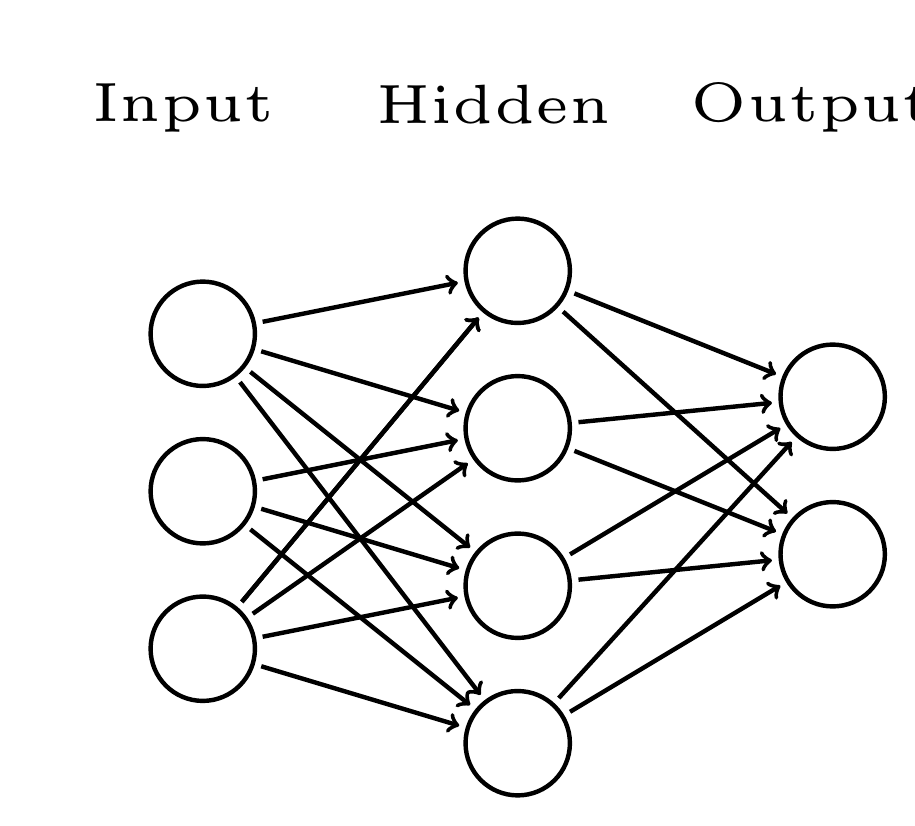
\begin{tikzpicture}[->,ultra thick,scale=4]
      \tikzstyle{every node}=[draw,shape=circle,scale=4]

      \node[draw=none,anchor=north,text width=0.1cm,font=\tiny] (input) at (-0.3,3.5) {Input};
      \node (v0) at (0,1.5) {};
      \node (v1) at (0,2) {};
      \node (v2) at (0,2.5) {};

      \node[draw=none,anchor=north,text width=0.1cm,font=\tiny] (input) at (0.6,3.5) {Hidden};
      \node (h0) at (1,1.2) {};
      \node (h1) at (1,1.7) {};
      \node (h2) at (1,2.2) {};
      \node (h3) at (1,2.7) {};

      \node[draw=none,anchor=north,text width=0.1cm,font=\tiny] (input) at (1.6,3.5) {Output};

      \node (o0) at (2,1.8) {};
      \node (o1) at (2,2.3) {};

      \draw (v0) -- (h0);
      \draw (v0) -- (h1);
      \draw (v0) -- (h2);
      \draw (v0) -- (h3);

      \draw (v1) -- (h0);
      \draw (v1) -- (h1);
      \draw (v1) -- (h2);
      \draw (v0) -- (h3);

      \draw (v2) -- (h0);
      \draw (v2) -- (h1);
      \draw (v2) -- (h2);
      \draw (v2) -- (h3);

      \draw (h0) -- (o0);
      \draw (h0) -- (o1);

      \draw (h1) -- (o0);
      \draw (h1) -- (o1);

      \draw (h2) -- (o0);
      \draw (h2) -- (o1);

      \draw (h3) -- (o0);
      \draw (h3) -- (o1);

    \end{tikzpicture}
  }
  \caption{A fully connected, feed-forward, artificial neural network with 3 input, 4 hidden and 2 output nodes.}
  \label{fig:ann}
\end{figure}

There are several ways to train an ANN, but the most common is to use an algorithm called \textit{backpropagation} to perform supervised learning.  The \textit{backpropagation} algorithm is so named because it propagates an error signal backward (from the output nodes toward the input nodes) through the network to assign blame and update connection weights.

Backpropagation can take a long time to converge to a solution, which may be a local optima and not a global one.  The computational complexity of backpropagation means that it can get prohibitively expensive to train large networks.  ANNs also typically grow in width rather than depth, when the model increases in complexity.  The reason for this is twofold:

\begin{enumerate}
 \item Adding a new layer, of same size, adds a lot more connections.  In a fully connected, feed-forward, network adding another layer of N nodes will create an additional $N^2$ connections, whereas adding another node only adds $N$ new connections.
 \item It is hard to meaningfully propagate an error signal through a very deep network.  If the weights are very small the gradient will be tiny at the start of the network.  If the weights are large, the gradients might be more reasonable, but we are likely to get stuck in a local minima of a highly multimodal landscape.
\end{enumerate}

In \cite{bengio09} Bengio makes a convincing case for why deep architectures are preferable to shallow ones.  The key point being that shallow networks are unable to efficiently encode certain functions.  These function are what the author calls \textit{highly varying functions}: functions where a piecewise-linear approximation of the function would require a large number of pieces.  In general this puts traditional ANNs at a disadvantage, and particularly so the ones being trained only with backpropagation.

\section{Restricted Boltzman Machines}

A Boltzman machine (BM) is a fully connected network of neuron-like units.  The connections are bidirectional and a stochastic process is used to determine whether a unit is on or not.  The number of connections in a BM makes them rather slow to train.  However, there exists an efficient learning algorithm\cite{hinton06} for a restricted BM (RBM): a BM where intra-layer connections are disallowed.

\begin{figure}[htb]
  \centering
  \scalebox{0.5}
  {
    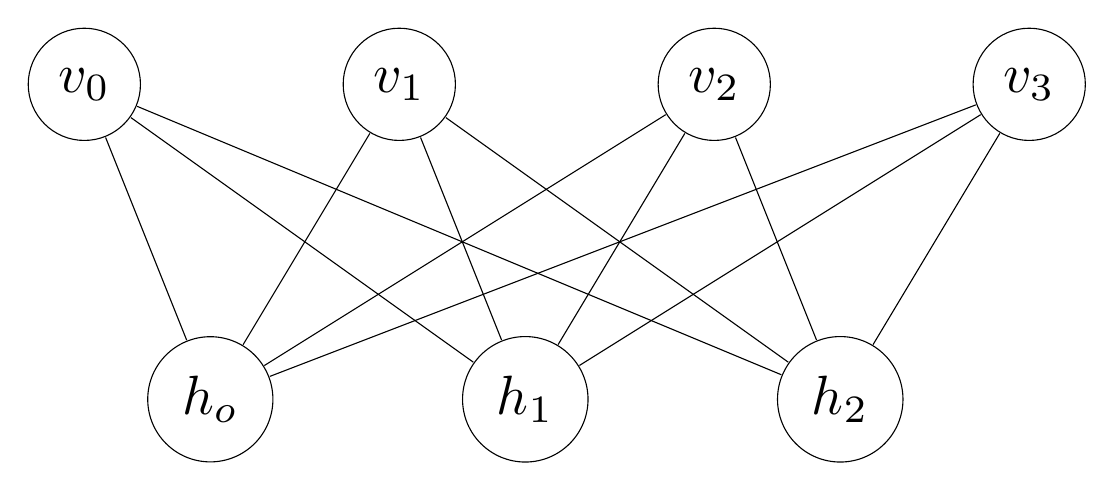
\begin{tikzpicture}[scale=4]
      \tikzstyle{every node}=[draw,shape=circle,scale=2]
      \node (h0) at (0.4,0) {$h_o$};
      \node (h1) at (1.4,0) {$h_1$};
      \node (h2) at (2.4,0) {$h_2$};

      \node (v0) at (0,1) {$v_0$};
      \node (v1) at (1,1) {$v_1$};
      \node (v2) at (2,1) {$v_2$};
      \node (v3) at (3,1) {$v_3$};

      \draw (v0) -- (h0);
      \draw (v0) -- (h1);
      \draw (v0) -- (h2);

      \draw (v1) -- (h0);
      \draw (v1) -- (h1);
      \draw (v1) -- (h2);

      \draw (v2) -- (h0);
      \draw (v2) -- (h1);
      \draw (v2) -- (h2);

      \draw (v3) -- (h0);
      \draw (v3) -- (h1);
      \draw (v3) -- (h2);
    \end{tikzpicture}
  }
  \label{fig:rbm}
  \caption{RBM with 4 visible and 3 hidden nodes.}
\end{figure}

Although RBMs might be unable to efficiently represent some distributions that can be compactly represented by a BM, it can be shown that an RBM, given enough hidden units, can represent any distribution\cite{le08}.  In addition, unless the RBM already perfectly models the training distribution, adding another hidden node (with correct weights and biases) always improves the model\cite{le08}.

The restricted Boltzman machine is so named because the energy metaphor is borrowed from physics.  In physics, the Boltzman distribution describes the fractional number of particles occupying a set of states with a given energy and temperature.  In our case, each input vector has a corresponding energy level.  During training this multi-dimensional energy landscape will be excavated to create ravines with clusters of training cases.  If the task is handwritten digit recognition then each digit class will map to a ravine in the energy landscape.  As in physics, the lower energy states are the most stable.

\subsection{RBM as a generative model}

A generative model is a model capable of randomly generating observable data, often using some hidden parameters.  Generative models are different from discriminative models in the sense that all the variables are modeled--through what is called a full probabilistic models.  A discriminative model, on the other hand, provides only a model for the target variables given the observed variables.  This means we can generate values for any variables in the model, whereas a discriminative model would only allow us to study how the target variables for are affected by the various observed variables.  Some examples, other than RBMs, of generative models are:

\begin{itemize}
 \item Gaussian, and other types, of mixture models.
 \item Hidden Markov Models
 \item Naive Bayes
\end{itemize}

There are many benefits of working with a generative model as opposed to a discriminative ones:

\begin{enumerate}
\item Generative models can learn low-level features, through unsupervised training, and they are capable of learning more parameters without overfitting.  In the discriminative case each training case only provides as many bits of information as are required to specify the label\cite{hinton06}, whereas in the generative case, each training case constrains the parameters by as many bits of information as are required to specify the input.
\item We can get insight into what the model has learned by sampling from the model.
\end{enumerate}

In terms of RBMs 2) means that the trained model can show its user what it believes in.

\subsection{Sampling from an RBM}

Sampling from the model is done using a process called Gibbs sampling.  Gibbs sampling is a Markov Chain Monte Carlo algorithm used to obtain random samples from the joint probability distribution of the model, when direct sampling is difficult.  We can use Gibbs sampling to get at the joint probability distribution of the model because we know the conditional distribution of each variable.

Gibbs sampling generates an instance from the distribution of each variable, one after another, conditional on the values of the other variables.  This sequence of samples makes up a Markov chain and the stationary distribution of this Markov chain is the desired joint distribution.

The conditional distribution of each variable is easy to get at because the hidden units are factorial--they are independent of one another, given the state of the visible units.

To perform Gibbs sampling, in the RBM, we clamp an input on the visible layer, which activates the hidden layer.  The hidden layer activation is in turn used to activate the visible layer.  This step is called reconstruction.  If we repeat this process sufficiently many times it will converge.

We can start the process off by sending in an instance of training data, e.g an example of a handwritten 9. This will seed the model in a favorable way and the process of Gibbs sampling will converge quicker.  In practice this means starting the model off inside the energy ravine containing known examples of other 9s and then having the model wander around until it settles on a state.  If we start the sampling process off with a random input vector, the process will take longer to converge and we are unable to affect which area of the energy landscape is explored to find a stable energy state.

\begin{figure}[htb!]
  \centering
  \includegraphics[width=\textwidth]{gibbs.png}
  \caption{Sampling from the model.}
  \label{fig:sampling}
\end{figure}

Figure \ref{fig:sampling} shows how the sampling process works in an RBM.  The process is started off with a sample of the visible units (created randomly, or preferably from a training case) and this is used to infer the state of the hidden units.  The state of the hidden units is then, in turn, used to reconstruct the values of the visible units.  Eventually this process will converge to a stable energy state--which we can interpret as something the model \textit{believes} in.

During sampling the individual activation probabilities are:

\begin{equation}
  \label{eq:h_state}
   P(h_j=1|v) = \sigma(b_j + \sum_{i=1}^n w_{i,j} v_i)
\end{equation}

and

\begin{equation}
\label{eq:v_state}
  P(v_i=1|h) = \sigma(a_i + \sum_{i=1}^m w_{i,j} h_j)
\end{equation}

Where $\sigma$ is a logistic sigmoid, \textit{v} denotes the visible layer and \textit{h} the hidden and $w_{i,j}$ is the weight matrix and $a_i$ and $b_i$ are biases.

\subsection{Training an RBM}

The learning rule for an RBM is:

\begin{equation}
\label{eq:training}
  \Delta w_{ij} = \epsilon(\langle v_ih_j\rangle_{data} - \langle v_ih_j\rangle_{model})
\end{equation}

Where the angle brackets denote the expectations under the distribution specified by the subscript that follows.

Because there are no connections between the hidden units, and between the visible units, in an RBM, it is very easy to get an unbiased sample of $\langle v_ih_j\rangle_{data}$.  As mentioned earlier this can be done with \ref{eq:h_state}, to get the state of the hidden units, and \ref{eq:v_state}, to get the state of the visible units.

Getting an unbiased sample of $\langle v_ih_j\rangle_{model}$ is however much more difficult.  It can be done using Gibbs sampling, but it would require an infinite number of steps.

The training algorithm \textit{constrastive divergence}, also called $CD_k$ where $\mathbf{k}$ is the number of steps used during Gibbs sampling, aims to solve this problem.  Contrastive divergence uses

\begin{equation}
\label{eq:cd}
  \Delta w_{ij} = \epsilon(\langle v_ih_j\rangle_{data} - \langle v_ih_j\rangle_{reconstruction})
\end{equation}

to approximate \ref{eq:training}.  Normally $CD_1$ is used, for training, where a single step of gibbs sampling is used.  It has been shown that this works well enough in practice, even though it looks pretty crude\cite{hinton06}.

\section{Autoencoders}

An autoencoder takes an input $\mathbf{x} \in [0,1]^d$ and maps it--the encoding part--to a representation in the hidden units, $\mathbf{y} \in [0,1]^{d'}$, through a deterministic mapping:
 $\mathbf{y} = s(\mathbf{W}\mathbf{x} + \mathbf{b})$ where $s$ is a non-linear function, e.g. a function from the Sigmoid family.

The latent representation $\mathbf{y}$, or \textit{code}, is then mapped back--the decoding part--into a reconstruction $\mathbf{z} = s(\mathbf{W'}\mathbf{y} + \mathbf{b'})$.  The transformation is completely analogue with the encoding step and $\mathbf{z}$ has the same shape as $\mathbf{x}$.  Note that ' does not mean that the vectors or matrices are transposed in this context.

Optionally we can let $\mathbf{W'} = \mathbf{W}^T$.  Using this constraint we say that the weights are \textit{tied}.  This same terminology is used for RBMs as well and in that context it means that we are using the same weights for discrimination and generation.

The parameters of the autoencoder $\mathbf{W}$, $\mathbf{b}$ and $\mathbf{b'}$ are optimized such that the average reconstruction error is minimized.  One way to do this would be to use the \textit{squared error} to guide the weight changes.

\begin{figure}[htb]
  \centering
  \scalebox{0.6}
  {
    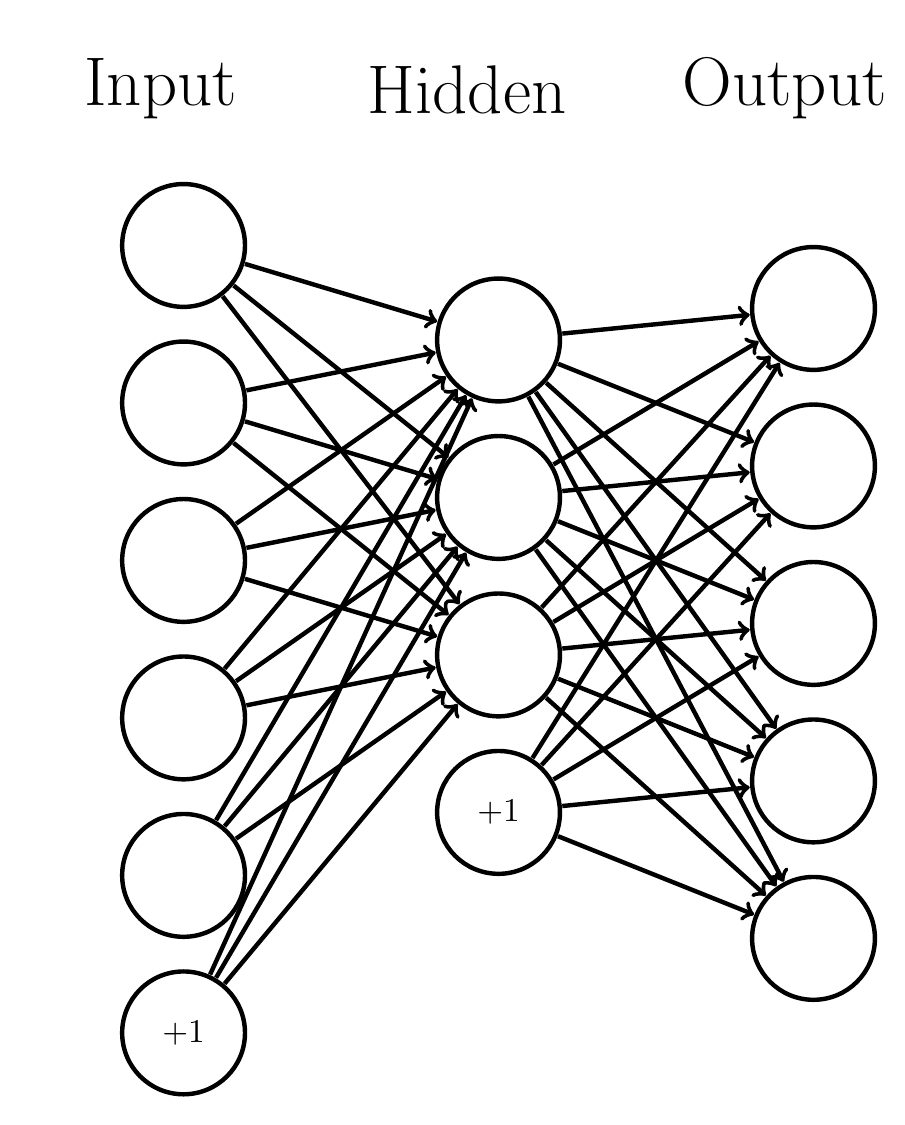
\begin{tikzpicture}[->,ultra thick,scale=4]
      \tikzstyle{every node}=[draw,shape=circle,minimum size=1.3cm,scale=4,text=,scale=0.3]

      \node[draw=none,anchor=north,text width=0.1cm,text=,scale=1,font=\huge] (input) at (-0.3,4.7) {Input};
      \node (v0) at (0,1.5) {+1};
      \node (v1) at (0,2) {};
      \node (v2) at (0,2.5) {};
      \node (v3) at (0,3) {};
      \node (v4) at (0,3.5) {};
      \node (v5) at (0,4) {};

      \node[draw=none,anchor=north,text width=0.1cm,text=,scale=1,font=\huge] (input) at (0.6,4.7) {Hidden};
      \node (h0) at (1,2.2) {+1};
      \node (h1) at (1,2.7) {};
      \node (h2) at (1,3.2) {};
      \node (h3) at (1,3.7) {};

      \node[draw=none,anchor=north,text width=0.1cm,text=,scale=1,font=\huge] (input) at (1.6,4.7) {Output};

      \node (o0) at (2,1.8) {};
      \node (o1) at (2,2.3) {};
      \node (o2) at (2,2.8) {};
      \node (o3) at (2,3.3) {};
      \node (o4) at (2,3.8) {};

      \draw (v0) -- (h1);
      \draw (v0) -- (h2);
      \draw (v0) -- (h3);

      \draw (v1) -- (h1);
      \draw (v1) -- (h2);
      \draw (v1) -- (h3);

      \draw (v2) -- (h1);
      \draw (v2) -- (h2);
      \draw (v2) -- (h3);

      \draw (v3) -- (h1);
      \draw (v3) -- (h2);
      \draw (v3) -- (h3);

      \draw (v4) -- (h1);
      \draw (v4) -- (h2);
      \draw (v4) -- (h3);

      \draw (v5) -- (h1);
      \draw (v5) -- (h2);
      \draw (v5) -- (h3);

      \draw (h0) -- (o0);
      \draw (h0) -- (o1);
      \draw (h0) -- (o2);
      \draw (h0) -- (o3);
      \draw (h0) -- (o4);

      \draw (h1) -- (o0);
      \draw (h1) -- (o1);
      \draw (h1) -- (o2);
      \draw (h1) -- (o3);
      \draw (h1) -- (o4);

      \draw (h2) -- (o0);
      \draw (h2) -- (o1);
      \draw (h2) -- (o2);
      \draw (h2) -- (o3);
      \draw (h2) -- (o4);

      \draw (h3) -- (o0);
      \draw (h3) -- (o1);
      \draw (h3) -- (o2);
      \draw (h3) -- (o3);
      \draw (h3) -- (o4);

    \end{tikzpicture}
  }
  \caption{An autoencoder with 5 input, 3 hidden, and 5 output nodes.  Bias nodes are included in the input and hidden layer.}
  \label{fig:ae}
\end{figure}

The gist of it all is that the autoencoder does its best to replicate the input.  The autoencoder shown in \ref{fig:ae} is perhaps the most common type, where the layer(s) between the input and output layer has a lower dimension.  This will force the autoencoder to learn a compressed representation of the input vector, which it then uses to create the output.  Intuitively, one would think that if the intermediary representation was of the same, or higher dimension, the autoencoder would simply learn the identity function.  Bengio et al. tackled this question in \cite{bengio07} and found that autoencoders with non-decreasing layer sizes also generalize well.  They do, however, speculate that this might be explained by their use of stochastic gradient decent and weight decay.  In other words in the general case, we might risk learning the identity function.

A final point about autoencoders is worth mentioning: if the autoencoder is built using only linear hidden units, i.e $\mathbf{s}$ is picked from the family of linear functions, then training the autoencoder is equivalent to performing principal component analysis (PCA).

\subsection{Denoising Autoencoders}

The denoising autoencoder is a stochastic version of the autoencoder.  Stochastic because the input is corrupted through some stochastic process.  The non-corrupted input is however used as a target for reconstruction.  The corruption process is performed by setting some, but not more than half, of the inputs to zero.  The denoising autoencoder is thus trying to perform two tasks:
\begin{enumerate}
\item Encode the input
\item Undo the effect of corruption
\end{enumerate}

The motivation behind the denoising autoencoder is to attempt to answer the question ``what properties should we demand of a good representation?''  Many come to mind, but the one investigated in \cite{bengio07} is ``robustness to partial destruction of the input''.  For high dimensional inputs, with redundant information (like in images), the representation is likely to depend on many factors along many dimensions and therefore likely be recoverable from partial observations.  The obvious example, mentioned in the paper, is our human ability to recognize objects which are partially covered up or corrupted in images.

\section{Deep Belief Networks}

\subsection{Using RBMs}

A deep belief network (DBN) can be created by stacking multiple RBMs.  When the input vector is processed by the first RBM its output is a new representation of the data.  This new representation can then be used as input to the RBM in the layer above.  The hope is that each RBM is better able to represent the data, by creating useful abstractions or simply removing noise.  In \cite{hinton06} Hinton shows that adding more layers in a DBN will always improve the model.  The use of the \textit{contrastive divergence} learning algorithm voids this guarantee, but it increases our confidence in the method to know that we can always improve the model by being patient enough in training each layer.

The way to train a DBN is to use a greedy layer-wise training algorithm.  Each layer, consisting of one RBM, is trained before we move on to train the next one.  By freezing the weights after we're done training each RBM we miss out on any positive effect that might be had by the coordinated tuning of weights in two, or more, adjacent layers.  One way to overcome this inefficiency of the greedy training approach is to fine-tune the network after the greedy training phase is done.  Fine-tuning can be done using the well-known backpropagation algorithm, or some other algorithm for gradient decent.  By seeding the backpropagation algorithm with a promising state (through pre-training) the following problems encountered using backpropagation in deep networks are solved\cite{hinton06reducing}:
\begin{enumerate}
\item If the initial weights are small the gradients in the earlier layers will be tiny and weight changes ineffectual.
\item If the initial weights are large the network typically gets stuck in poor local minima.
\end{enumerate}

When the initial weights are just right, gradient decent works quite well.

\subsection{Using autoencoders}

A deep belief network can also be created by stacking multiple (denoising) autoencoders.  The process is entirely analogous to the situation with RBMs.  First the network is trained using unsupervised pre-training and then fine-tuned using an algorithm like backpropagation.  In \cite{bengio07} DBNs using stacked denoising autoencoders were found to perform as good, or better, than DBN networks of stacked RBMs, on the MNIST dataset.

\subsection{As an autoencoder}

Another related type of network can be found in \cite{hinton06reducing}.  In this paper, which is about dimensionality reduction of data using ANNs, three RBMs of dimensions 2000-1000, 1000-500 and 500-30 are trained using a greedy unsupervised approach, as discussed earlier.  The weights are then \textit{unrolled} to create a new network of structure 2000-1000-500-30-500-1000-2000, which is then fine-tuned using backpropagation.  This network is itself an autoencoder and is referred to as a \textit{deep autoencoder}.

\section{Convolutional Neural Networks}

The first convolutional neural network (CNN) was described in Fukushima's seminal paper on the Neocognitron\cite{fukushima}.  The modern terminology was not used in this paper, but the key principles are the same.  Inspired by the work done by Hubel and Wiesel, on the cat's visual cortex\cite{hubel}, the goal was to create a biologically plausible ANN to explore image recognition (specifically, images of digits).  One of the key insight in Fukushima's paper is that feature detection should be modular and location invariant: we should re-use the same structure in order to detect one feature in the image, regardless of the coordinates of the feature within the image.  In implementational terms, in regard to an ANN, this means we should re-use weights to detect features.

\subsection{What is convolution}

The term convolution is taken from the field of image processing.  In image processing, to convolve an image, with a filter (also called kernel), means to apply the filter to each pixel in the image.  A filter is created by defining weights of neighbor pixels to a center pixel.

An example can be seen in figure \ref{fig:convolution}.  Here the emboss kernel is used.  Using the emboss kernel the filtered image will represent the rate of color change at each location in the original image.  The emboss kernel only has non-zero elements on the main diagonal, and the center element is zero.  Thus, the value of the center pixel is $4 * 0 + 2 * -4 = -8$.
\begin{figure}[htb!]
  \centering
  \includegraphics[width=\textwidth]{convolution.jpg}
  \caption{Example of convolution using the emboss kernel.}
  \label{fig:convolution}
\end{figure}

By using different filters, we can process the image to achieve various effects.  Some common filters used result in sharpening, blurring or edge detection.

The use of convolution in ANNs is quite analogous: the filter is a feature detector. The sum, of products of pixel values and weights, is not used to create a new center pixel, but instead expresses the probability that the feature being detected is present at the given location in the picture.  Thus, the result of convolving an image with a filter is a matrix of probabilities, also called a feature map.  By convolving the image with many filters we can create several feature maps.  If we denote the k-th feature map at a given layer as $h^k$, which is determined by the weights $W^k$ and bias $b_k$ then the feature map $h^k$ is:

\begin{displaymath}
  h^{k}_{ij} = \sigma((W^k * x))_{ij} + b_k
\end{displaymath}

Where * means matrix convolution, and not multiplication, and $\sigma$ is some non-linear function, typically selected from the sigmoid family.

\subsection{Pooling}

Pooling is another important component of CNNs.  Each unit in the pooling layer has a receptive field in the convolution layer below.  The role of the unit is to aggregate the values in its receptive field, in some meaningful way.  The feature maps created in the convolution layer is partitioned into non-overlapping rectangles, and for each sub-region, the pooling value is calculated.

There are various types of pooling, but the most common ones are max and mean pooling.  For max pooling the output is simply the maximum value in the receptive field.  And for mean-pooling it is the mean value of all the units in the receptive field.

Pooling serves two purposes:

\begin{enumerate}
\item Reduction of computational complexity, for upper layers of the network.
\item Provide translational and deformational invariance.
\end{enumerate}

Since pooling provides increased robustness, in terms of the position of features within an image, it has proven to be a good way of reducing the dimensionality of the intermediary representations.

If we refer back to the work done by Hubel and Wiesel the convolution step used for feature extraction corresponds to the work done by the \textit{simple cells} and the pooling operation to the work done by the \textit{complex cells} found in the visual area V1.

\begin{figure}[htb]
  \centering
  \includegraphics[width=\textwidth]{mylenet.png}
  \caption{Model of LeCun's convolutional network LeNet}
  \label{fig:mylenet}
\end{figure}

In figure \ref{fig:mylenet} we get a descriptive view of how a CNN works, with alternating convolution and sub-sampling (max-pooling) layers.  In layer $\mathbf{S1}$ we can see 4 feature maps, describing the probabilities that 4 different features are present at various locations of the image.  $\mathbf{C1}$ is a sub-sampling layer performing pooling.  $\mathbf{C1}$ then feeds into $\mathbf{S2}$ which creates new feature maps based on more abstract features.  At the very top of the network, in LeNet, we find a fully connected multi-layer perceptron (MLP) with logistic regression.

In figure \ref{fig:mylenet} we can also see how the receptive field of each detector increases in size as we move toward the to of the network.  For instance if the first convolutional layer uses filters with receptive fields which are 4x4 in size, representing the receptive field of \textit{simple cells}.  The max pooling layer might look at say a 3x3 region of the resultant feature map, and in terms of the original image, each \textit{complex cell} would then have receptive field of size $(4 + 3 - 1)^2$ pixels from the input image, or $(rank(\mathbf{S1}) + rank(\mathbf{C1}) - 1)^2$.  Where $rank(A) = n\ \Leftrightarrow$ A is an $N\times N$ matrix.

\subsection{Use of convolutional neural networks}

For a long time (until Hinton published \cite{hinton06} in 2006) the only viable option for creating deep artificial neural networks was to use a convolutional network.  Deep fully connected networks trained using backpropagation were computationally intractable, but the CNNs were not.  There are several reasons for this:

\begin{enumerate}
 \item The filters are small.  It is therefore not very computationally intensive to find the correct weights used to detect a feature.
 \item The complexity of the network can be controlled by choosing how many features to use at each level.
 \item The sub-sampling layers do not need training at all.
 \item The sub-sampling layers provide a reduction in dimensionality, decreasing the computational load.
 \item Shared weights reduces duplication of knowledge throughout the network.
\end{enumerate}

The ideas used in convolutional networks are sound, so they have not fallen out of favor.  On the contrary, they are very scalable and produce state-of-the-art results.  There are several ways to put any additional computational power to good use:
\begin{itemize}
 \item Detect more features.
 \item Adjust the size of the filters.  Smaller filters are more computationally intensive, but afford a higher level of detail.
 \item Add more layers.
\end{itemize}

CNNs are primarily used in machine vision, because the statistics of the image is the same everywhere (a given feature is equally likely to appear anywhere in the input image) making translational invariance very important.

\subsection{Multi-scale Convolutional Network}

In \cite{farabet} a CNN is created, which is scale invariant, for the purpose of scene parsing.  The scene parsing task consist of identifying and labeling the objects making up an image.  In practice this means assigning an object class to each pixel in the image e.g. sky, road or person.

The importance of scale invariance, in regards to this task, is obvious: it is desirable for a ``small person'', i.e. a person in the background of the image, to be identified as a person even if the training set only contains images where the persons appear in the foreground.

The problem of scale invariance can be solved by extending the concept of weight sharing over locations, to sharing weights over scales.  The weights are shared among different CNNs.  During classification the image is scaled--3 different sizes are used in the paper--and each version is sent to one CNN.  The final feature vector represents the concatenation of the feature vectors from the 3 CNNs.

\begin{figure}[htb]
  \centering
  \includegraphics[width=\textwidth]{mymscnn.png}
  \caption{Depiction of generation of feature vector for various scales.}
  \label{fig:mscn}
\end{figure}

Figure \ref{fig:mscn} shows how feature extraction in the multi-scale convolutional network is done.  The model parameters, $\theta$, is shared between all the networks.

\subsection{Multi-column deep neural network}
In \cite{ciresan} and \cite{ciresan2} a multi-column deep convolutional network (MCDNN) is used to improve the state-of-the-art on several classification tasks, the most famous of which are the MNIST and NORB dataset.  Traditional CNNs, with randomly initialized weights, are created and all of them trained either on the same training sets or distorted variants.  The final classification is done with a democratic vote between the CNNs, referred to as columns in the paper.

Max pooling is used to create a winner-take-all effect where only the winner neurons receive training.  The authors argue that this represents a biologically plausible mechanism where the ever decreasing number of changes per time interval lead to reduced energy consumption.

In order to speed up training the entire system is optimized to run on a graphics processing unit (GPU), a processor dedicated to rendering graphics. The authors estimate that using GPUs leads to an increase in computational power of around 50-100x.  Furthermore, this additional processing power removes the need for pre-training completely.  The network is trained through no other means than an online version of backpropagation (weight updates after each training case).

This system is the first one able to achieve human-competitive results on the MNIST dataset.  Humans are reported to achieve error levels of 0.2\%, the MCDNN system manages 0.23\%


\subsection{Convolutional Deep Belief Network}

In \cite{lee} a convolutional deep belief network is created.  Recall that what separates a deep belief network from other kinds of deep networks is that it is a generative model, able to generate observable data.  There are several reasons that make the combination of convolutional and deep belief networks desirable:
\begin{itemize}
 \item The effect of training on unlabeled data is greater in belief networks.
 \item The lack of mechanisms like weight-sharing and pooling for RBM based deep belief networks makes training on large input images computationally intractable in practice.
 \item Deep belief networks are able to do inference both top down and bottom up, i.e. they are able to infer missing data.
\end{itemize}

The building blocks in the deep convolutional belief network is the convolutional RBM (CRBM).  A CRBM is similar to a regular RBM, but with a few key differences:

\begin{itemize}
 \item The hidden layer of the RBM is really two layers:
   \begin{itemize}
           \item A \textit{detection layer} which performs convolution.
            \item A \textit{a pooling layer} which performs pooling.
          \end{itemize}
 \item The detection layer has $\mathbf{K}$ groups, made up of $\mathbf{N_H \times N_H}$ hidden units.  And each group has a $\mathbf{N_W \times N_W}$ filter associated with that group.
 \item To sample from the visible units we use convolution instead of propagating the activation of the input layer.
\end{itemize}

Max-pooling was only intended for feed-forward architectures so a new variant called probabilistic max-pooling is used.  A regularization step is also used in order to force sparsity, because the model in the paper is overcomplete and does not generalize well without the regularization.

\begin{figure}[htb]
  \centering
  \includegraphics[width=\textwidth]{mycdbn.png}
  \caption{Depiction of a convolutional RBM with probabilistic max pooling.}
  \label{fig:crbm}
\end{figure}

\newpage

Figure \ref{fig:crbm} show a CRBM, where $\mathbf{W^k}$ is the k-th filter and $\mathbf{h^k_{i,j}}$ is a hidden unit in the k-th group.

\section{Implementation}

At the very beginning of the semester we wanted to ``implement an RBM, to get familiar with the terminology, and see if we could replicate the results on the MNIST dataset''.  Software engineers are notorious for being unable to estimate how long something is going to take, but our estimate of two weeks of effort, turned out to be several orders of magnitude too low.

The main problem was that the source material we had on hand was entirely unsatisfactory, given our background.  The only resources available were scientific papers and an implementation written in Python, where all the code was executed on the GPU.

There is little doubt that we could have implemented the system correctly if we could only understand all the math in the research papers on deep belief networks, or Boltzman machines, but these proofs are well out of our reach.  We had hoped that we could use these networks, and find interesting applications and results, without understand all the details of how and why they work.

At \href{http://deeplearning.net/tutorial}{deeplearning.net} there is a Python implementation of a DBN using stacked RBMs.  This code, and the tutorial itself, is maintained by Yoshua Bengio's group at the university of Montreal.  Bengio is one of the leading researcher in the field of deep learning.

We thought we could reference this code base in order to get answers to any question we had after reading the research papers.  The problem we encountered were two-fold:

\begin{enumerate}
 \item Python is a dynamically typed language.
 \item Python allows operator overloading.
 \item The implementation relies heavily on Theano, a library for running code on GPUs.
\end{enumerate}

ANNs are typically implemented using operations on vector and matrices.  Point 1) and 2) meant that we often found ourselves in the following situation, when trying to read the code: is this a scalar, a vector, or a matrix?  In some cases scalar values were even aggregated into vectors just for performance reason (an operation could then be performed in parallel on each element of the vector on the GPU).  3) meant we had to dive into, and decipher, code in the GPU library in order to find out what was really going on.

This process was very time consuming, and often we realized, after some time, that we would probably never find the answer we were looking for.
\subsection{Haskell}

One of the authors had been dabbling with Haskell, a pure, functional language for the better part of a year.  Haskell seemed to be a well-suited language for implementing an RBM, and both authors were eager to explore the world of functional programming--which has received quite a bit of attention lately.  The following properties of Haskell were especially attractive to us in regards to this project:
\begin{enumerate}
 \item Haskell is very ``high level'', making it possible to get a lot done with few lines of code.
 \item Great performance.
 \item Easy to write highly parallel code, due to immutable data structures, and high quality abstractions for the parallellization of programs.
 \item Good libraries for matrix multiplication, relevant for implementing common operations found in ANNs.
 \item CUDA/OpenCL bindings (making it possible to perform computations on GPUs).
\end{enumerate}

We knew we wanted, or at least would benefit greatly from, points 2), 3) and 5) because we wished to work with large networks and datasets.  While not unwarranted, these concerns were perhaps a bit premature.

After two weeks time we ended up abandoning Haskell and going with Java.  Java might not be as sexy, but it's a tried and true platform capable of delivering on points 4) and 5), while not being entirely unsatisfactory in regards to points 2) and 3).  Haskell is a very complex language, and many of the abstractions found in the libraries are very complex as well.  We were learning a lot, and having a great time, but had to remind ourselves that this was a project intended for exploring AI, and not programming languages.  Getting everything re-implemented in Java took about two days.  The problem was never how much code we had to write, but what to write in the first place.

\subsection{What we implemented}

We managed to implement an RBM, with all that entails (contrastive divergence, Gibbs sampling etc).  This RBM seems to work correctly.

Some of the papers we read, including the deeplearning tutorial, had a softmax regression layer at the very top of the artificial neural network.  Softmax regression is a multivariate logistic regression method.  Plain logistic regression is used when the labels are mutually exclusive and binary.  With our usage of the MNIST dataset the use of softmax regression means that each example will only have one label, and the probabilities of all the labels will be normalized, so they sum to one.  Our implementation of softmax regression also seems to be correct.

We have the mechanisms in place to stack however many RBMs we want, but we're not entirely sure if it is done correctly or not.

\subsection{Results}

We used the MNIST dataset for all tests of the system.  The MNIST dataset consist of 60 000 training cases, of handwritten digits, and 10 000 test cases.  This is a very large training set and we often used a subset of the dataset, instead of all of it, when we just wanted to debug the system.

All of the results described below are taken from memory, well after the fact, and represents nothing else than the results we obtained while working on implementing and improving the system.  These results do not represent ``good science'', but they were produced consistently by the system and they are all we have.

\subsubsection{A single RBM}

We managed to implement a single RBM, and train it using contrastive divergence on the MNIST dataset.  Training took around 2 minutes per epoch.  An epoch means training on all of the training cases. We initially trained for 10 epochs, but found we could get away with less. When the system was used for classification the best results were had when we only trained for 2 epochs.

This very simple model, with 250 hidden nodes, managed an error rate consistently between 10-15\% on the full MNIST dataset.

\begin{figure}[htb!]
  \centering
  \includegraphics[width=\textwidth]{filters.png}
  \caption{A view of the filters in our RBM.  The filters represent various feature detectors.}
  \label{fig:filters}
\end{figure}

Figure \ref{fig:filters} shows the filters of the RBM.  These feature detectors give a pretty clear indication that the RBM we implemented is doing work related to handwritten digit recognition.  Each filter is created by making an image out of all the weights connecting all the input nodes (784, in these 28x28 images) to one hidden unit, and then scaling the values to represent them as a grey scale image.

\subsubsection{Stacked RBMs}

The next step was to see what happened when we stacked two RBMs.  Our initial attempt achieved an error rate of 30\%.  We tried several configurations, the best result was achieved with 3 stacked RBMs and was just above 20\%.

\subsubsection{Softmax Regression}

Softmax regression is full-blown learning algorithm in its own right and when we ran it on the full MNIST dataset we managed an error rate of 7.5\%.

Our best results was obtained when we used one RBM and put a softmax regression layer above it.  We managed an error rate of 6.5\% using this approach.

% BEGIN RECEIVE ORGTBL results
\begin{table}[htb!]
\centering
\begin{tabular}{|l|r|}        \hline
Approach & Error Rate (\%) \\ \hline
Single RBM & 10-15 \\         \hline
Two RBMs & 30\ \\             \hline
Three RBMs & 20 \\            \hline
Softmax regression & 7.5 \\   \hline
RBM + Softmax & 6.5 \\        \hline
\end{tabular}
\caption{Results achieved during system implementation on the MNIST dataset.}
\label{tbl:results}
\end{table}
% END RECEIVE ORGTBL results
\begin{comment}
#+ORGTBL: SEND results orgtbl-to-latex :splice nil :skip 0
| Approach           | Error Rate (\%) |
| Single RBM         |          10-15 |
| Two RBMs           |            30\ |
| Three RBMs         |             20 |
| Softmax regression |            7.5 |
| RBM + Softmax      |            6.5 |
\end{comment}


\subsection{Discussion}

Our results are summarized in table \ref{tbl:results}.  We were very excited when we achieved, what we considered to be, such a low error rate on our first test, using only a single RBM.  Obviously, we were very disappointed, and confused, when the error rate went up as we added more layers.

The idea, of course, is that each layer is going to present a better and better view of the data to the next layer, making its job easier.  The very last layer would have an easy job of classifying the training cases indeed.

This is one of the major drawbacks of working in computer science: when something does not work as expected, is your approach wrong, or does the system simply contain a bug?  We spent endless amounts of time on code review--how do you even write unit or regression tests for something like this? We never found any serious bugs.

Instead we thought maybe we were lacking some critical feature. For instance Hinton, in\cite{hinton06}, makes use of something called a \textit{softmax group}.  A softmax group is a group of units, constrained so only one unit is active.  The softmax group is used to ensure that during training only one label unit is set during reconstruction.  When we tried to implement this, the error rate was no better than chance.  We were never able to figure out if our understanding was wrong, if there was a bug in the implementation, or if the components--picked from different papers and the deeplearning tutorial--simple weren't compatible.

In \cite{hinton06} Hinton says, in his conclusion, that it isn't clear if \textit{fine-tuning} is needed at all, or if, perhaps, the computational resources are better spent training an ensemble of networks, a larger network, or on a larger training set.  This, and similar remarks, led us to believe that the greedy pre-training (contrastive divergence) was the be-all and end-all of training these networks, and that \textit{fine-tuning}, using for instance backpropagation, would only slightly decrease our error rate.  As a consequence we spent a lot of time trying to find bugs in our implementation and understanding.

In \cite{bengio07} the point is made that the result of pre-training is finding a promising area of the solution space, from which a gradient descent algorithm can find the optimal solution.  In \cite{ciresan} and \cite{ciresan2} a deep network is trained entirely without pre-training, with very impressive results.  The work done in \cite{ciresan}, and \cite{ciresan2}, is with convolutional networks--networks that are less complex, and thus perhaps more amenable to training without pre-training. Nevertheless, an interesting question is raised as to exactly how important pre-training is.

When we decided to pull the plug, on the project, our plan was to run a few tests using backpropagation in order to determine the exact effect of pre-training.  Could we do without pre-training?  Perhaps the higher error rate seen when stacking multiple RBMs is normal, and something like backpropagation or another fine-tuning algorithm (like wake-sleep or up-down) is completely necessary for networks of those sizes.

We also did not experiment enough with different network sizes.  We used, mostly, architectures very similar to what we'd seen in papers working with the MNIST dataset, but our network was not identical to any of them.  It is unlikely, but nonetheless possible, that we could have achieved better results by using a different network size.  The fact of the matter is that we felt, and still feel, that we don't understand deep belief networks deeply enough.  This led us to focus--perhaps more than we should have--on bug hunting in our system and understanding instead of on experimentation.

\subsection{Concluding remarks}

We are very disappointed with the results of our implementation efforts.  The state of the field is such that it's not clear, yet, exactly what works and what does not and which components fit where.  We found it very difficult to mix and match components and insights from different papers and then evaluate the results.  It was hard for us to say what was normal, and where more features would improve performance, and what was simply broken due to lack of understanding or bugs.

\section{Future work}

In \cite{farabet} the task of scene labeling is tackled.  Scene labeling in itself is a difficult task, but it is further complicated by the difficulty of creating good datasets.

In order to create such a dataset one has to send a human out into the world to take pictures.  These pictures then have to be processed--correctly segmented and labeled--by humans.  Often this is done through services like Amazon's Mechanical Turk, an out-sourcing service where you can pay humans to solve repetitive tasks.  Needless to say this entire process is costly, in terms of time and money.

One of the characteristics of all the deep networks we have encountered is their ability to sponge up training data.  We've seen time and again how the error rate decreases monotonically with the size of the training set.  This has resulted in various strategies to use existing training data to manufacture more.  Most of these strategies boil down to applying various transformations to the training data, e.g. slight deformation, rotation, etc.

It is our hope that we can solve the tension existing between the desire for vast and tailor-made datasets and the costly nature of procuring them.

We want to see if we can use modern graphic engines to generate training data for use in machine vision.  Specifically we want to investigate if we can use data generated from a virtual world to:

\begin{enumerate}
 \item Replace training data generated from the real world entirely.  Using these datasets only for testing.
 \item Augment training data from the real world.
\end{enumerate}

We think 2) is doable, and are hoping for 1).  If it's not possible now, Moore's law basically guarantees that it will be possible in the near future.

In terms of the scene labeling task the datasets generated from the virtual world have a few interesting properties:

\begin{itemize}
 \item We can easily change the time of day to generate images under different lighting conditions.
 \item We can easily change the weather.
 \item The number of labels we can use is only limited by the amount of art assets available.
 \item It is much easier to create hierarchical labels, expressing relations like is-part-of.
 \item We can generate endless amounts at very low cost.
 \item We can generate images that might not be possible to get in the real world.
 \item Its easy to generate datasets for different user-agents.  The different user agents will have their viewpoint at different elevations and pitch (e.g the viewpoint of the navigation system of a car vs a drone).
\end{itemize}


\begin{figure}[htb!]
  \centering
  \includegraphics[width=\textwidth]{myce3ss.jpg}
  \caption{A screen capture of art assets rendered using the graphics engine CryEngine 3.}
  \label{fig:cryEngine}
\end{figure}

As can be seen in figure \ref{fig:cryEngine} the state of the art in computer graphics is quite impressive. It's not hard to imagine how machine vision systems can benefit from training on such images.

\section{Conclusion}

Various types of deep neural networks are at the bleeding edge of many classification tasks.  There are many factors which make them attractive classifiers, but chief among them are perhaps:
\begin{enumerate}
\item The ability to train on raw data, avoiding the need for complex feature engineering.
\item Scalability, combined with the ever-increasing availability of computational resources.
\item The ability to tackle a diverse range of tasks without relying on domain knowledge.
\item Performance can be improved, greatly, by doing unsupervised training on readily available unlabeled data.
\end{enumerate}

We have focused on image processing, partly because we find this application most interesting, but also because the literature itself favors this task.  The reason for this favoritism is not only due to flights of fancy, but because certain mechanisms, like weight-sharing and max-pooling work very well when the input data is contiguous (e.g. as image data is, or a contiguous sound wave).  Another reason is that the imaging tasks represent real challenges due to both the size and high dimensionality of the input data, making the task a worthy research subject.

In general we can say that the neural networks encountered all excel, to various degrees, on tasks that humans are also good at.  This means they're good at tasks like voice recognition, speech-to-text and vision, but perform very poorly if we try to use them as a calculator.

The obvious value of any improvements to tasks like machine vision has lead to a situation where there is a lot more back and forth between academia and industry than was is usual for AI research.  Google is currently using deep belief networks to power their voice-to-text engine found in the Android operating system.  In \cite{ng} Andrew Ng teamed up with Google to run deep learning, on an object recognition task, using a cluster of 1000 machines for a total for 16000 cores.  The model has one billion connections.

Deep networks also powered Microsoft's recent demonstration of real-time translation of speech, where the speech was synthesized using a model of the speaker's own voice.  The net result was a presentation where the speaker spoke English and the audience heard the speaker speak Chinese, in his own voice.  The demonstration of this technology is well worth a \href{http://www.youtube.com/watch?v=Nu-nlQqFCKg}{look}.

The short distance between theory and practice for this technology, makes it especially interesting to work with.

\bibliographystyle{plain}
\bibliography{references}

\end{document}
